\section{Methods}
	\begin{multicols*}{2}
		[\subsection{\gls{SRS} analysis}
		\gls{SDLC} starts with eliciting the \gls{SRS}, noted by the stakeholders. As stakeholders use their own language to state their requirements, it is observed to be very often ambiguous and confusing to analyze and subsequently design the desired solution. On one side we only focus on \gls{SRS} requirement document which follows the IEEE-STD-830 standard in a textual form. In the other side \gls{NLP} concepts are found to be helpful for the analysis. \gls{NLP} system processes the data written in natural language in an intelligent manner and generates an information which is comparatively easier to analyze.\cite{Tripathy}]
		Using \gls{NLP} can help in:
		\begin{itemize}
			\item the syntax of natural language
			\item the lexical context of the words
			\item the semantic components which construct the literal meaning of a sentence
			\item the pragmatic components which construct non-literal meaning of a sentence
			\item the parser generating the phrase tree structure of a sentence.
		\end{itemize}
		\gls{POST} is a semantic analysis approach and deals with assigning one or more \gls{POS} to a given word. The different types of \gls{POS} are,
		\begin{itemize}
			\item Noun (names): a word or lexical item denoting any abstract (abstract noun: e.g. home) or concrete entity (concrete noun: e.g. house); a person (police officer, Michael), place (coastline, London), thing (necktie, television), idea (happiness), or quality (bravery). Nouns can also be classified as count nouns or non-count nouns; some can belong to either category. The most common part of speech; they are called naming words.
			\item Pronoun (replace or again placed): a substitute for a noun or noun phrase (them, he). Pronouns make sentences shorter and clearer since they replace nouns.
			\item Adjective (describes, limits): a modifier of a noun or pronoun (big, brave). Adjectives make the meaning of another word (noun) more precise.
			\item Verb (states action or being): a word denoting an action (walk), occurrence (happen), or state of being (be). Without a verb a group of words cannot be a clause or sentence.
			\item Adverb (describes, limits): a modifier of an adjective, verb, or another adverb (very, quite). Adverbs make language more precise.
			\item Preposition (relates): a word that relates words to each other in a phrase or sentence and aids in syntactic context (in, of). Prepositions show the relationship between a noun or a pronoun with another word in the sentence.
			\item Conjunction (connects): a syntactic connector; links words, phrases, or clauses (and, but). Conjunctions connect words or group of words.
			\item Interjection (expresses feelings and emotions): an emotional greeting or exclamation (Huzzah, Alas). Interjections express strong feelings and emotions.
			\item Article (describes, limits): a grammatical marker of definiteness (the) or indefiniteness (a, an). The article is not always listed among the parts of speech. It is considered by some grammarians to be a type of adjective or sometimes the term 'determiner' (a broader class) is used.
		\end{itemize}
		Identification of all these \gls{POS} makes the task of \gls{NLP} simpler.
		
		Following Fillmore’s idea of defining a universal set of cases and Nan Niu’s variation structure, Wang et al. introduce a set of extended dimensions for conceptualizing the functional variability structure\cite{5381217}. An \gls{EFRF} is composed by 10 different semantic cases. Thus, the following variation dimensions for an \gls{EFRF} are considered.
		\begin{itemize}
			\item Agentive defines the agent whose activities will occur in \gls{EFRF}’s affairs. For example, $\{\mbox{student}\}_{Agentive}$
			“do homework”.
			\item Action defines the main action of the activity. For
			example, “TA” $\{\mbox{mark}\}_{Action}$.
			\item Objective defines the object affected by the activity.
			For example, “mark” $\{\mbox{homework}\}_{Objective}$.
			\item Agentmod defines the feature of agent. For example,
			{Senior}Agentmod $\{\mbox{student}\}_{Agentive}$.
			\item Objmod defines the feature of object. For example,
			$\{\mbox{c++}\}_{Objmod} \{\mbox{homework}\}_{Objective}$.
			 \item Locational defines the location where the \gls{EFRF} affairs occur. For example, “do homework” $\{\mbox{at home}\}_{Locational}$.
			 \item Temporal defines the duration or frequency of the
			 \gls{EFRF}’s activity. For example, “mark homework” $\{\mbox{every Sunday}\}_{Temporal}$.
			 \item  Manner defines the way or tool by which the
			 \gls{EFRF}’s activity is performed. Some examples are,
			 “access Internet” via $\{\mbox{Ethernet, Wireless}\}_{Manner}$,
			 “mark assignment” through $\{\mbox{Internet}\}_{Manner}$.
			 \item Goal defines the goal of the \gls{EFRF}’s activity. For example, “do homework carefully” $\{\mbox{in order to get an A}\}_{Goal}$.
			 \item Constraint defines the requirement and constraint
			 that make the activity occur. For example, “do
			 homework on-line” if $\{\mbox{access Internet}\}_{Constraint}$.
		\end{itemize}
		This extended set reflects most grammatical features
		that are associated with functional requirements description;
		hence it can serve as a framework of categories that helps
		analysts understand the variation points, i.e. what can vary,
		of the \gls{EFRF}. The systematical and clear definition of these
		variable points can help the effectiveness of software product line's functional variability modeling. 

		\begin{minipage}{0.9\linewidth}
			\centering
			\begin{figure}[H]
				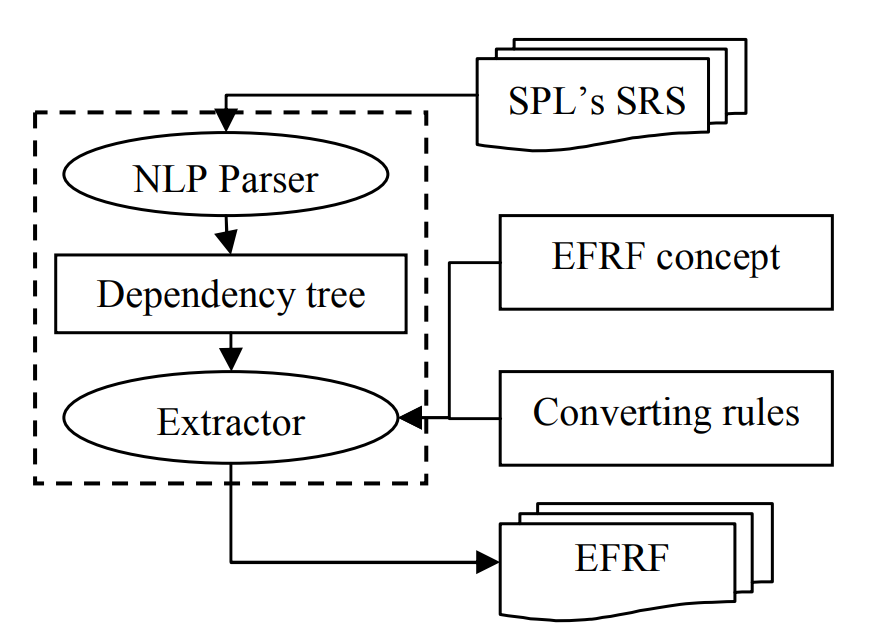
\includegraphics[width=\linewidth]{Architecture}
				\caption{Architecture}
			\end{figure}
		\end{minipage}
		
		First the NLP Parser is the Stanford Parser \cite{stanfordParser} as the NLP parser. It can generate dependency trees to express the
		grammatical relations in sentences. The grammatical relations are arranged in a hierarchy, rooted with the most generic relation named “dependent”. Altogether, the hierarchy
		contains 48 grammatical relations. The whole hierarchy of
		the grammatical relations is given in \cite{Marneffe}.
		The second step is the Extractor, where the grammatical relations are converted into \gls{EFRF}s by converting rules which are introduce by \cite{5381217}. In this step, \gls{EFRF}s are merged which express the
		same functional requirements. If two \gls{EFRF}s describe the same
		activity, then they will be merged by combining their cases. 
		
	\end{multicols*}


\begin{minipage}{\linewidth}
	\begin{multicols*}{2}
		[
		\vspace{6 mm}
		\subsection{Semantic Analyzer}
		Despite C provides constructs that map to machine instructions, it also provides enough abstraction above \gls{asm} for developers to finish their work independently of platform  on which their C program runs.]
		Despite the abstraction mentioned above, C is known for the deftness in which it allows to developers to write programs with bugs. Despite there is no runtime error detection and just a little static analysis, in C the developers trust entirely. The C language is low-level enough despite its abstraction, so developers take advantage of supposition about the root architecture.  
		Back in time, the C standard was written in two of the design principles: the ability to develop a non-portable code and the trust in the programmer\cite{AmericanNationalStandardsInstitute:1990:RAC:533966}. Such principles also work together to create complex, platform-dependent bugs. The possible subtlety of C bugs makes them an ideal formalization candidate, as subtle bugs can often be found only by more thorough means.
		
		In this article, a formal semantics of \gls{MISRA} C is presented that is to be used to find bugs. "Formal semantics for realistic programming languages are large and complicated. This raises the question of validating these semantics: how can we make sure that they correctly capture the expected behaviors?" questions Blazy-Leroy in his "Mechanized semantics for the Clight subset of the C language" \cite{Blazy}. He writes how a subset of the C language can be formalized. Many uses of C in embedded or critical applications mandate strict coding guidelines restricting programmers to a “safer” subset of C \cite{HATTON2004465}. A well-known example is \gls{MISRA} C \cite{MISRA2004}. \gls{MISRA} C and Clight \cite{Blazy} share some restrictions (such as structured \textit{switch} statements with \textit{default} cases at the end), but otherwise differ significantly. For instance, \gls{MISRA} C prohibits recursive functions, but permits all uses of \textit{goto}. More generally, the restrictions of \gls{MISRA} C and related guidelines are driven by software engineering considerations and the desire for tool-assisted checking, while the restrictions of Clight stem from the desire to keep its formal semantics manageable.
	\end{multicols*}
\end{minipage}

\begin{minipage}{\linewidth}
	\begin{multicols*}{2}
		[
		\vspace{6 mm}
		\subsection{Consistency Check}
		Even though diverse techniques for requirements analysis and model derivation have been developed, problems still remain in this process, mainly related with the ambiguity, incompleteness and inconsistency of the documented requirements. Documenting high-quality software requirements \cite{Ieee1998} that efficiently support the follow-up software analysis and design remains a classical challenge to the requirements engineering research community. ]
		
		In a current state-of-the-practice there exist tools that allow formalization of software requirements in a semi-automatic way. There
		are also tools for checking the consistency of a given set of formalized requirements. However, there is a very limited support for
		\gls{MIS} identification, i.e., the identification of the sources of the inconsistency of an inconsistent set of requirements in the domain
		of temporal logics. \cite{Bendik:2017:CCR:3092703.3098239} focuses on this gap and in particular, it aims to address the following research questions:
		\begin{itemize}
			\item What are the differences between temporal logics and logics for which efficient \gls{MIS} enumeration algorithms already
			exist, and what techniques used in the latter setting can be
			applied also in the former one?
			\item Are there some domain specific properties of temporal
			logics, e.g., negation normal form of linear temporal logic formulas, that 	can be exploited by a singe \gls{MIS} extraction algorithms?
			\item Which consistency checking approaches are the most suitable to be employed by \gls{MIS} enumeration algorithms?
		\end{itemize}
		 
		The main contributions of the research direction, both those that
		have been already achieved and those that are expected, are the
		following. \cite{Bendik:2017:CCR:3092703.3098239} provides novel algorithms for online \gls{MIS} enumeration which are applicable to any type of input logic. These algorithms are especially suitable for temporal logics, as they tend to minimize the number of performed
		consistency checks during their execution which is the
		most relevant criterion in the case of temporal logics domain.
	\end{multicols*}
\end{minipage}

